% Provenance (never printed): the institutions strand of ../economics_series.md (grade 9: three natural experiments, the
% Koreas, the Germanys, China 1978; what differs: ownership, who decides, free prices, contract enforcement; income
% against corruption; a correlation is not yet a cause). Brief: sources/book1/BRIEFS.md, g9-06. The WGI chart is refused
% (licence): the corruption measure is the World Bank Enterprise Surveys' bribery incidence (IC.FRM.BRIB.ZS, via WDI).
% The cause question across countries is left to the Year 3 volume.
% Chart data: figdata/grade-9/06-institutions-and-prosperity (Maddison KOR, PRK, CHN; WDI bribery and income; the
% problem's invented valleys). Ledger: g9:germany-east-west-1991, -1996, g9:lin-1992, g9:china-reform-1978.
\chapter{Why Some Countries Are Rich: Institutions}\label{ch:g9:institutions-and-prosperity}

\begin{openingchart}{GDP per person in South Korea and North Korea, 1940--2022, in dollars of 2011 (times-ten
scale). There is no estimate for North Korea from 1944 to 1989: its line is missing there.}{Maddison Project
Database 2023 (Bolt and van Zanden)}
\begin{tikzpicture}
\begin{semilogyaxis}[omtimesten, xmin=1940, xmax=2022, ymin=500, ymax=100000, ytickten={3,4,5},
  xtick={1940,1960,1980,2000,2020}, xlabel={Year}, ylabel={Dollars of 2011 per person}, legend pos=north west,
  unbounded coords=jump]
\addplot[omDef, thick] table[x=year, y=south] {figdata/grade-9/06-institutions-and-prosperity/out/koreas.csv};
\addplot[omThm, thick] table[x=year, y=north] {figdata/grade-9/06-institutions-and-prosperity/out/koreas.csv};
\draw[guide] (axis cs:1948,500) -- (axis cs:1948,15000);
\node[anchor=north west, font=\scriptsize, rotate=90] at (axis cs:1949.5,1900) {two states, 1948};
\legend{South Korea, North Korea}
\end{semilogyaxis}
\end{tikzpicture}
\end{openingchart}

% figdata: koreas (1940 south 1975, north 2624; 2022 south 41321, north 1569; ratio 26.3)
In 1940 the north of Korea produced more per person than the south: 2,624 dollars against 1,975. After
1948 the peninsula was two states with the same language and the same history, which had started from
similar \omterm{def:g7:households:income}{incomes}. In 2022 South Korea produced 41,321 dollars per person, and North Korea 1,569: the South produced
26 times as much per person.

\begin{recall}
\omterm{def:g8:gdp:gdp-per-person}{GDP per person} is measured in dollars of fixed purchasing power (\cref{ch:g6:living-standards}). A
country that grows by $5\,\%$ a year doubles its \omterm{def:g7:households:income}{income} in about 14 years
(\cref{ch:g8:growth-and-compounding}). In a \omterm{def:g7:markets-and-prices:market}{market}, \omterm{def:g7:money:price}{prices} move until the \omterm{def:g7:demand-and-supply-first-look:quantity-demanded}{quantity demanded} equals the
\omterm{def:g7:demand-and-supply-first-look:quantity-supplied}{quantity supplied} (\cref{ch:g7:markets-and-prices}).
\end{recall}

\section{One people, two systems: the Koreas}

\begin{definition}[Natural experiment]\label{def:g9:institutions-and-prosperity:natural-experiment}
A \emph{natural experiment}\index{natural experiment} is an event that splits similar people into groups
that live under different conditions, as an experiment would, without anyone having planned it as an
experiment.
\end{definition}

The division of Korea is a \omterm{def:g9:institutions-and-prosperity:natural-experiment}{natural experiment}. The land, the climate and the people were alike on both
sides of the line. What differed was the set of rules: who owned farms and factories, who decided what to
produce, how \omterm{def:g7:money:price}{prices} were set.

\begin{omfigure}
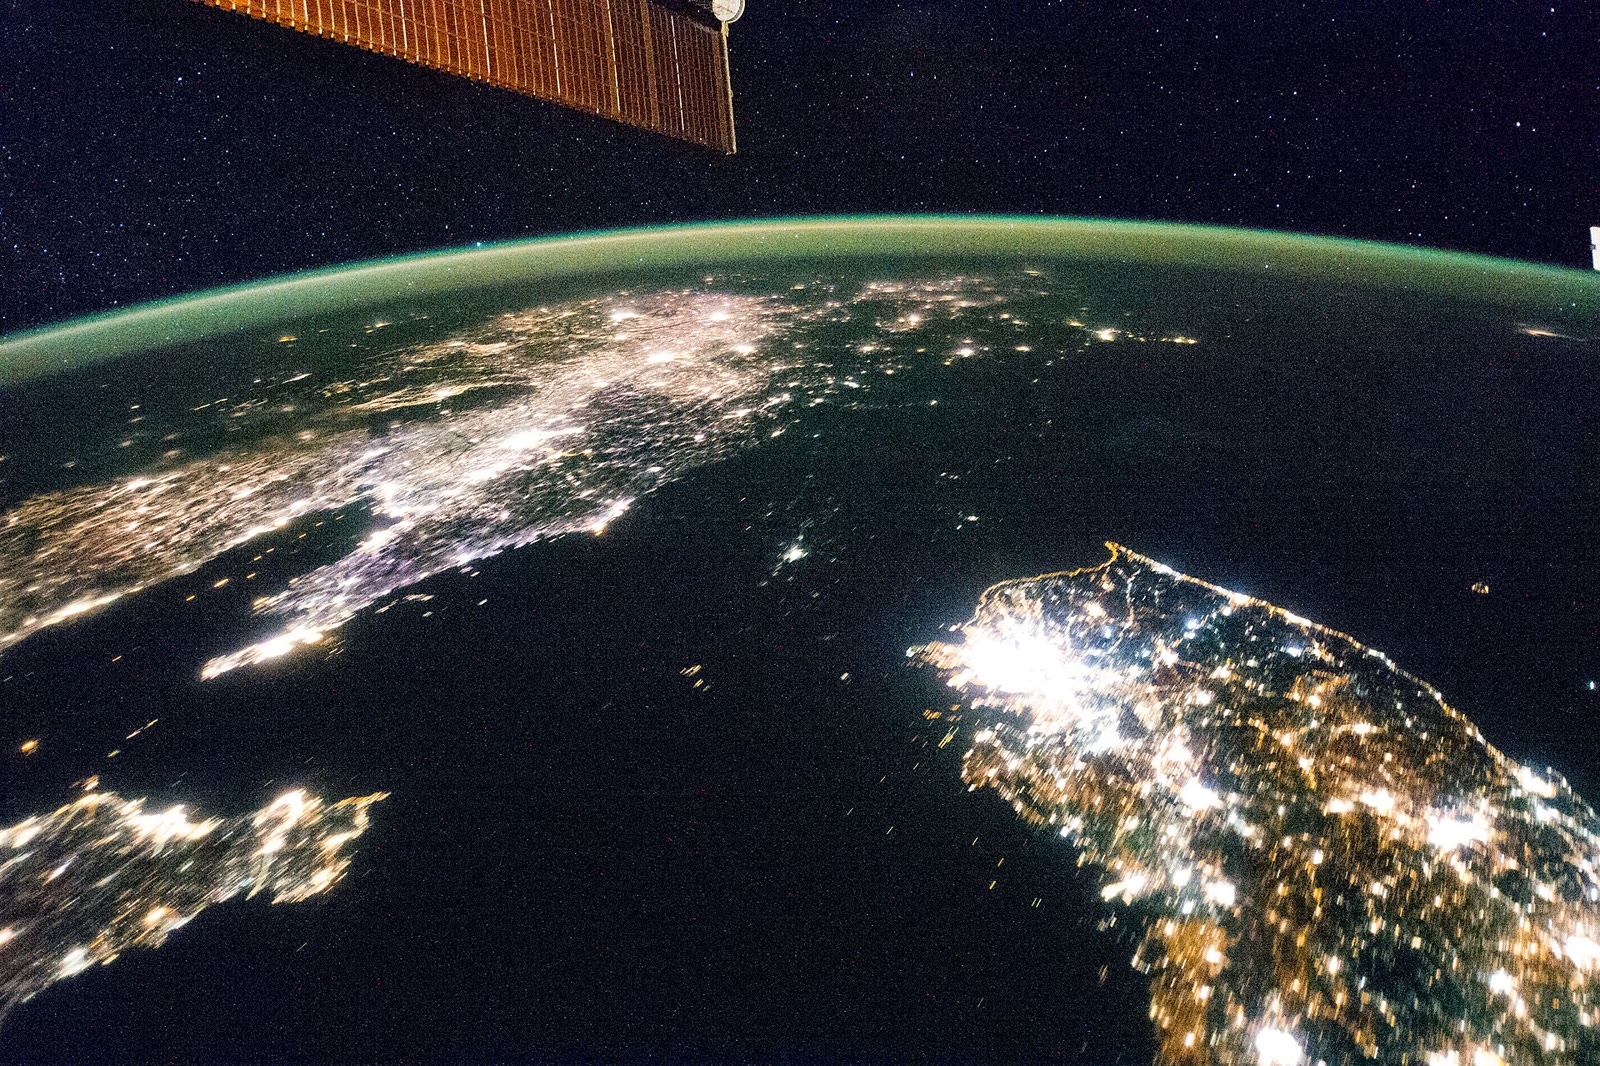
\includegraphics[width=0.62\linewidth]{images/book1/photos/g9-institutions-korea-at-night.jpg}

{\small The Korean peninsula at night, seen from the International Space Station in 2014, looking north.
South Korea, lower right, is bright with the lights of its cities; North Korea, above it, is almost dark.
The lights at the top left are in China.}
\end{omfigure}

\begin{definition}[Planned economy]\label{def:g9:institutions-and-prosperity:planned-economy}
In a \emph{planned economy}\index{planned economy} the state owns most farms and \omterm{def:g7:firms:firm}{firms} and decides what they
produce, in what quantities, and at what \omterm{def:g7:money:price}{prices} they sell.
\end{definition}

\begin{definition}[Market economy]\label{def:g9:institutions-and-prosperity:market-economy}
In a \emph{market economy}\index{market economy} most farms and \omterm{def:g7:firms:firm}{firms} belong to people and companies, who
decide what to produce, and most \omterm{def:g7:money:price}{prices} are set by buyers and sellers in \omterm{def:g7:markets-and-prices:market}{markets}.
\end{definition}

North Korea has a \omterm{def:g9:institutions-and-prosperity:planned-economy}{planned economy}. South Korea has a \omterm{def:g9:institutions-and-prosperity:market-economy}{market economy}, in which the state also played a large part in
its first decades.

% figdata: facts kor_south_growth_90_22 3.5, kor_north_growth_90_22 -1.4
From 1990 to 2022, South Korea's \omterm{def:g8:gdp:gdp-per-person}{GDP per person} grew by $3.5\,\%$ a year on average; North Korea's fell, by
$1.4\,\%$ a year.

\section{The two Germanys}

From 1949 to 1990 Germany was also two states: a \omterm{def:g9:institutions-and-prosperity:market-economy}{market economy} in the west, a \omterm{def:g9:institutions-and-prosperity:planned-economy}{planned economy} in the
east. The two shared a language and a history.

\begin{record}[Germany, 1949--1990]
% ledger: g9:germany-east-west-1991, g9:germany-east-west-1996
In 1990 the two states became one. In 1991, the first full year after unification, East Germany's \omterm{def:g8:gdp:gdp-per-person}{GDP per
person} was $40\,\%$ of West Germany's. Under the west's rules and \omterm{def:g9:exchange-rates-and-purchasing-power:currency}{currency} it rose fast, to somewhat above $60\,\%$ in
1996, and then stayed near that level until at least 2001 (European Commission, 2002).
\end{record}

\section{China before and after 1978}

% figdata: china (1950 799, 1978 1744, 2022 19238; growth 2.8 % 1950-78, 5.6 % 1978-2022)
\begin{omchart}{China's GDP per person, 1950--2022, in dollars of 2011 (times-ten scale). The dashed line
marks 1978, when the rural reforms began.}{Maddison Project Database 2023 (Bolt and van Zanden)}
\begin{tikzpicture}
\begin{semilogyaxis}[omtimesten, xmin=1950, xmax=2022, ymin=500, ymax=50000, ytickten={3,4},
  extra y ticks={50000}, extra y tick labels={},
  xtick={1950,1960,1970,1978,1990,2000,2010,2022}, xlabel={Year}, ylabel={Dollars of 2011 per person},
  height=0.45\linewidth]
\addplot[omDef, thick] table[x=year, y=gdppc] {figdata/grade-9/06-institutions-and-prosperity/out/china.csv};
\draw[black!60, dashed] (axis cs:1978,500) -- (axis cs:1978,50000);
\end{semilogyaxis}
\end{tikzpicture}
\end{omchart}

China gives a third experiment, with the same people at two times. Until 1978, farms were worked by
collectives: the harvest belonged to the group and was shared out, whatever each family did, and most of it
had to be sold to the state at fixed \omterm{def:g7:money:price}{prices}. From 1978, families could farm their own plots, deliver a fixed
quantity to the state, and keep or sell the rest. Later, \omterm{def:g7:firms:firm}{firms} and \omterm{def:g7:markets-and-prices:market}{markets} spread to the rest of the
economy.

From 1950 to 1978 China's \omterm{def:g8:gdp:gdp-per-person}{GDP per person} grew by $2.8\,\%$ a year on average; from 1978 to 2022, by $5.6\,\%$
a year, so that it was multiplied by 11.

\begin{record}[China after 1978]
% ledger: g9:lin-1992, g9:china-reform-1978
A study of China's provinces found that the return of farms to families accounted for about half of the
growth of farm output from 1978 to 1984; higher \omterm{def:g7:money:price}{prices} paid by the state accounted for part of the rest
(Lin, 1992).
\end{record}

\section{What differs: ownership, decisions, prices, contracts}

\begin{definition}[Institution]\label{def:g9:institutions-and-prosperity:institution}
An \emph{institution}\index{institution} is a rule of the game of a society, written or not, that shapes
what people can do and what they can expect from others: laws, courts, property, customs.
\end{definition}

\begin{definition}[Property right]\label{def:g9:institutions-and-prosperity:property-right}
A \emph{property right}\index{property right} is the right of an owner to use a thing, to keep what it earns,
and to sell it.
\end{definition}

\begin{definition}[Contract enforcement]\label{def:g9:institutions-and-prosperity:contract-enforcement}
\emph{Contract enforcement}\index{contract enforcement} is the means, usually courts, by which a person can
make another keep a promise they agreed on, such as paying for goods delivered.
\end{definition}

\begin{omfigure}
\begin{tikzpicture}[font=\small, every node/.style={align=center, text width=4.6cm}]
  \node[font=\small\bfseries] at (0,2.9) {Planned economy};
  \node[font=\small\bfseries] at (5.4,2.9) {Market economy};
  \node[draw, fill=omThm!8, minimum height=1.1cm] at (0,2) {The state owns farms and firms};
  \node[draw, fill=omDef!8, minimum height=1.1cm] at (5.4,2) {People and companies own them};
  \node[draw, fill=omThm!8, minimum height=1.1cm] at (0,0.7) {A plan decides what is made};
  \node[draw, fill=omDef!8, minimum height=1.1cm] at (5.4,0.7) {Owners decide, guided by prices};
  \node[draw, fill=omThm!8, minimum height=1.1cm] at (0,-0.6) {The state sets prices};
  \node[draw, fill=omDef!8, minimum height=1.1cm] at (5.4,-0.6) {Buyers and sellers set prices};
  \node[draw, fill=omThm!8, minimum height=1.1cm] at (0,-1.9) {Orders from above};
  \node[draw, fill=omDef!8, minimum height=1.1cm] at (5.4,-1.9) {Contracts enforced by courts};
\end{tikzpicture}

{\small Four differences between the two kinds of economy.}
\end{omfigure}

\begin{model}{Institutions and income}
\assumes People work, invest and trade more when they keep what they earn and when promises made to them
are kept.
\predicts With the same people and the same land, rules that secure property, let owners decide and let
\omterm{def:g7:money:price}{prices} move give a higher \omterm{def:g6:living-standards:income-per-person}{income per person} over decades.
\tested The Koreas, the two Germanys, and China after 1978 (this chapter).
\breaks Across countries, the link is a \omterm{def:g9:institutions-and-prosperity:correlation}{correlation}: geography, history and culture also differ. And fast
growth has also happened where property was not secure for everyone; the volume for the third university
year returns to the question of cause.
\end{model}

\section{Across countries: a correlation, not yet a cause}

\begin{definition}[Correlation]\label{def:g9:institutions-and-prosperity:correlation}
Two quantities are \emph{correlated}\index{correlation} when they tend to move together across cases: when
one is high, the other tends to be high (or low).
\end{definition}

% figdata: facts brib_n 168; below 5000: 33 countries, median 14.4; above 30000: 54 countries, median 2.6
\begin{omchart}{Share of firms asked for at least one bribe, in percent, against GDP per person at
purchasing-power parity (dollars of 2021, times-ten scale): one dot per country, latest survey from 2016 to
2025 (168 countries).}{World \omterm{def:g8:banks-saving-interest:bank}{Bank} Enterprise Surveys and World Development Indicators (IC.FRM.BRIB.ZS and
NY.GDP.PCAP.PP.KD)}
\begin{tikzpicture}
\begin{semilogxaxis}[omincomex, xmin=700, xmax=200000, ymin=0, ymax=55, width=0.85\linewidth,
  height=0.48\linewidth, xlabel={GDP per person (dollars of 2021, times-ten scale)},
  ylabel={Firms asked for a bribe (percent)}]
\addplot table[x=income, y=bribery]
  {figdata/grade-9/06-institutions-and-prosperity/out/bribery_income.csv};
\end{semilogxaxis}
\end{tikzpicture}
\end{omchart}

In the 33 countries with less than 5,000 dollars per person, the middle country had $14.4\,\%$ of its \omterm{def:g7:firms:firm}{firms}
asked for a bribe; in the 54 countries with more than 30,000 dollars, $2.6\,\%$. Bribery and poverty are
\omterm{def:g9:institutions-and-prosperity:correlation}{correlated}. The chart does not say which causes which, if either: bribes may keep a country poor, by
making \omterm{def:g7:firms:firm}{firms} pay to work; poverty may breed bribes, when officials are badly paid; or something else, such
as a long history of war, may cause both.

\begin{measure}[A correlation across countries]
A chart of dots shows a \omterm{def:g9:institutions-and-prosperity:correlation}{correlation} when the dots lie along a band rather than in a shapeless cloud. The
bribery chart is close to a cloud: among the poorest countries the share runs from almost none to almost
half of all \omterm{def:g7:firms:firm}{firms}. The pattern shows in the middle values, $14.4\,\%$ against $2.6\,\%$, more than in
what the eye sees. To
read it as a cause, one needs to know that nothing else differs between the countries on the left and
those on the right, and that the arrow does not go the other way. A \omterm{def:g9:institutions-and-prosperity:natural-experiment}{natural experiment}, such as the
Koreas, comes closer, because so much else is the same on both sides.
\end{measure}

\section{Exercises}

\begin{exercise}[$\star$]\label{exo:g9:institutions-and-prosperity:1}
Use the opening chart. Which part of Korea produced more per person in 1940? Which in 2022?
\end{exercise}

\begin{exercise}[$\star$]\label{exo:g9:institutions-and-prosperity:2}
In 2022 South Korea produced 41,321 dollars per person and North Korea 1,569. How many times as much did the
South produce per person?
\end{exercise}

\begin{exercise}[$\star$]\label{exo:g9:institutions-and-prosperity:3}
China's \omterm{def:g8:gdp:gdp-per-person}{GDP per person} was 1,744 dollars in 1978 and 19,238 in 2022. By how many times was it multiplied?
\end{exercise}

\begin{exercise}[$\star$]\label{exo:g9:institutions-and-prosperity:4}
Over the 44 years from 1978 to 2022, a \omterm{def:g8:growth-and-compounding:growth-rate}{growth rate} of $5\,\%$ a year multiplies an amount by $8.56$, $5.5\,\%$
by $10.55$ and $6\,\%$ by $12.98$. Use these numbers and exercise 3 to find China's average \omterm{def:g8:growth-and-compounding:growth-rate}{growth rate}
between two of them.
\end{exercise}

\begin{exercise}[$\star\star$]\label{exo:g9:institutions-and-prosperity:5}
From 1990 to 2022 (32 years), South Korea's \omterm{def:g8:gdp:gdp-per-person}{GDP per person} went from 13,874 to 41,321 dollars and North
Korea's from 2,456 to 1,569. Over 32 years, $3.5\,\%$ a year multiplies an amount by $3.01$, and a fall of
$1.4\,\%$ a year by $0.64$. Compute the two ratios and say which rate fits each country.
\end{exercise}

\begin{exercise}[$\star\star$]\label{exo:g9:institutions-and-prosperity:6}
Use the bribery chart. Around what share of \omterm{def:g7:firms:firm}{firms} are asked for a bribe in the poorest countries, and in the
richest? Give the middle values from the text.
\end{exercise}

\begin{exercise}[$\star\star$]\label{exo:g9:institutions-and-prosperity:7}
A country lets farmers sell, at \omterm{def:g7:markets-and-prices:market-price}{market prices}, what they grow beyond a fixed delivery to the state. What does
the model predict for farm output? What did happen in China after 1978?
\end{exercise}

\begin{exercise}[$\star\star$]\label{exo:g9:institutions-and-prosperity:8}
In 1991, East Germany's \omterm{def:g8:gdp:gdp-per-person}{GDP per person} was $40\,\%$ of West Germany's. How many times as much did West Germany
produce per person? What was the answer in 1996, when the share was about $60\,\%$?
\end{exercise}

\begin{exercise}[$\star\star$]\label{exo:g9:institutions-and-prosperity:9}
Describe an observation that would contradict the model of this chapter.
\end{exercise}

\begin{exercise}[$\star\star\star$]\label{exo:g9:institutions-and-prosperity:10}
In an invented table of six countries, the three with good courts are all on the coast and rich; the three
with poor courts are all far from the sea and poor. Do good courts make countries rich, according to this
table? What else could explain it?
\end{exercise}

\begin{exercise}[$\star\star\star$]\label{exo:g9:institutions-and-prosperity:11}
A country takes its farms from their owners and makes them state farms, with fixed \omterm{def:g7:money:price}{prices} for the harvest.
What does the model predict for farm output over the next decades? Why?
\end{exercise}

\begin{exercise}[$\star\star\star$]\label{exo:g9:institutions-and-prosperity:12}
Why does the bribery chart, on its own, not show that bribery makes countries poor? Give two other
explanations of the pattern.
\end{exercise}

\section{Problem: Two Valleys}

\begin{problem}[{Weekend problem --- two invented valleys with the same land and people but different rules
for harvests, their output over twenty years, and a reform in the poorer valley}]
\label{pb:g9:institutions-and-prosperity:1}
Everything in this problem is invented. Two valleys have the same soil, climate and people. Each produces
1,000 dalens per person in year 0. In valley A each family keeps its harvest, after a fixed rent. In valley B
the whole harvest is pooled and shared equally, whatever each family does.

\medskip
\noindent\textbf{Part I --- The rules.}
\begin{enumerate}
  \item In valley A, a family works harder and grows 100 dalens more. How much more does it keep?
  \item In valley B, with 100 families, one family grows 100 dalens more. How much more does it receive?
  \item Which valley does the model of this chapter predict will grow faster? Why?
\end{enumerate}

\medskip
\noindent\textbf{Part II --- Twenty years.} Valley A grows by $3\,\%$ a year and valley B by $1\,\%$.
Round to the nearest dalen.
\begin{enumerate}[resume]
  \item Compute output per person in each valley in year 1 and in year 2.
  \item In year 20 valley A produces 1,806 dalens per person and valley B 1,220. Check that $1.03^{20}$ is
        about $1.806$.
  \item How many times as much does valley A produce per person in year 20? By what percentage is it ahead?
\end{enumerate}

\medskip
\noindent\textbf{Part III --- A reform.} In year 20 valley B adopts valley A's rules. From then on it grows by
$5\,\%$ a year, while valley A keeps growing by $3\,\%$.
\begin{enumerate}[resume]
  \item Compute both valleys' output per person in years 21 and 22.
  \item By what percentage is valley A ahead in year 22?
  \item Each year, by what factor does the ratio of A to B shrink? (Compute $1.03 \div 1.05$.)
  \item Valley A's lead was $48\,\%$ in year 20. What lead is half of it?
  \item In year 29, valley A produces 2,357 and valley B 1,893; in year 30, 2,427 and 1,988. In which year
        is the lead halved for the first time?
  \item How many years after the reform is that? Why does the gap close faster in percent than in dalens?
\end{enumerate}
\end{problem}
